\documentclass[11pt]{article}


\usepackage{fullpage}
\usepackage{graphicx}
\usepackage{amsmath}
\usepackage{amssymb}
\usepackage{amsthm}
\usepackage{fancyvrb}

\newcommand{\myname}{Mehshan Mustafa}

\newenvironment{theorem}[2][Theorem]{\begin{trivlist}
\item[\hskip \labelsep {\bfseries #1}\hskip \labelsep {\bfseries #2.}]}{\end{trivlist}}
\newenvironment{lemma}[2][Lemma]{\begin{trivlist}
\item[\hskip \labelsep {\bfseries #1}\hskip \labelsep {\bfseries #2.}]}{\end{trivlist}}
\newenvironment{exercise}[2][Exercise]{\begin{trivlist}
\item[\hskip \labelsep {\bfseries #1}\hskip \labelsep {\bfseries #2.}]}{\end{trivlist}}
\newenvironment{problem}[2][Problem]{\begin{trivlist}
\item[\hskip \labelsep {\bfseries #1}\hskip \labelsep {\bfseries #2.}]}{\end{trivlist}}
\newenvironment{question}[2][Question]{\begin{trivlist}
\item[\hskip \labelsep {\bfseries #1}\hskip \labelsep {\bfseries #2.}]}{\end{trivlist}}
\newenvironment{corollary}[2][Corollary]{\begin{trivlist}
\item[\hskip \labelsep {\bfseries #1}\hskip \labelsep {\bfseries #2.}]}{\end{trivlist}}
\newenvironment{solution}{\begin{proof}[Solution]}{\end{proof}}
\newenvironment{idea}[2][Proof Idea.]{\textit{#1} #2}



\parindent0in
\pagestyle{plain}
\thispagestyle{plain}

\newcommand{\dated}{\today}
\newcommand{\token}[1]{\langle \text{#1} \rangle}

\begin{document}

\textbf{Introduction to the Theory of
Computation}\hfill\textbf{\myname}\\[0.01in]
\textbf{Chapter 3: The Church-Turing Thesis}\hfill\textbf{\dated}\\
\smallskip\hrule\bigskip

\begin{problem}{3.9}
Let a $k$-PDA be a pushdown automaton that has $k$ stacks. Thus a $0$-PDA is an NFA and a $1$-PDA is a conventional PDA. You already know that $1$-PDAs are more powerful (recognize a larger class of languages) than $0$-PDAs.
\end{problem}

\begin{problem}[Part]{a}
Show that $2$-PDAs are more powerful than $1$-PDAs.
\end{problem}

\begin{proof}
A $2$-PDA can simulate any $1$-PDA by using only one of it's stacks. Therefore, $2$-PDAs can recognize all the languages that are recognized by $1$-PDAs. Additionally, we show that $2$-PDAs can also recognize more languages, which are not recognized by $1$-PDAs. For example, the language $A = \{a^nb^nc^n \ | \ n \geq 0 \}$. The language $A$ is not a context free language\footnote{Example 2.36, Chapter 2.}, but we can construct a $2$-PDA to recognize $A$ as follows:
\begin{enumerate}
\item Read and push $a$'s on both stacks until a $b$ is read.
\item Once a $b$ is read, match it with an $a$ by popping an $a$ from the first stack. Keep reading and matching any subsequent $b$'s. Reject if the number of $a$'s and $b$'s are not equal.
\item Next, match $c$'s with $a$'s on the second stack. Accept if the number of $a$'s and $c$'s are equal, reject otherwise.
\item In above steps, also make sure the input string is in $a^*b^*c^*$.
\end{enumerate}
\end{proof}

\begin{problem}[Part]{b}
Show that $3$-PDAs are not more powerful than $2$-PDAs.
\end{problem}

\begin{proof}
To show that $3$-PDAs are not more powerful than $2$-PDAs, we show how two stacks can be used to simulate a Turing machine tape.
\begin{enumerate}
\item Consider an arrangement of the two stacks, where the two stacks are placed horizontally next to each other. The right hand side (RHS) stack grows to the right, whereas the left hand side (LHS) stack grows to the left.
\item Mark the end of stacks by pushing special symbols before any input is processed. Let $\pi$ and $\lambda$ be two distinct symbols, which are not part of the input language:
\begin{enumerate}
\item Push $\pi$ on the LHS stack.
\item Push $\lambda$ on the RHS stack.
\end{enumerate}
\item The read/write head is always at the top of the RHS stack. For now, assume that the input symbols are available on the RHS stack. Later we show how to load input string on the RHS stack.
\begin{enumerate}
\item To read, pop from the RHS stack.
\item To write, push on the RHS stack.
\end{enumerate}
\item Move left and right are simulated by push and pop operations on the two stacks:
\begin{enumerate}
\item To move right, pop a symbol from the RHS stack and push it to the LHS stack.
\item To move left, pop a symbol from the LHS stack and push it to the RHS stack.
\end{enumerate}
\item Special cases for the left-most and right-most end of the tape:
\begin{enumerate}
\item If $\pi$ is popped from the RHS, then this indicates that the head is at the left-most position of the tape. In this case, push $\pi$ back on the LHS stack and read again.
\item If $\lambda$ is popped from the RHS, then this indicates that the head is at the right-most position of the tap. To simulate infinite tape on the right, in this case the input symbol is assumed to be the blank and the $\lambda$ is pushed back on the RHS stack. The written symbol is pushed on the LHS stack. 
\end{enumerate}
\end{enumerate}

\begin{center}
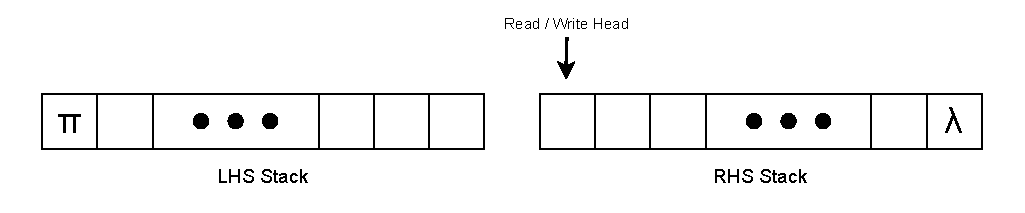
\includegraphics[scale=1.0]{Figures/Problem3.9.pdf} \\
Configuration of the two stacks. RHS stack grows to the right, \\ and the LHS stack grows to the left. The ends of LHS and RHS \\ stacks are marked by the symbols $\pi$ and $\lambda$ respectively.
\end{center}

Load input string on the RHS stack as follows:
\begin{enumerate}
\item Push $\pi$ on the LHS stack, and $\lambda$ on the RHS stack to mark their ends.
\item Repeatedly, read a symbol from the input, push it on the LHS stack and non-deterministically go to step 3.
\item Pop symbols from LHS stack and push them on the RHS stack. Once the LHS stack is emptied, non-deterministically go to step 4.
\item Process the input string on the RHS stack as discussed earlier.
\end{enumerate}
\end{proof}

\end{document}